%\documentclass{article}
\documentclass[conference,10pt,twocolumn]{./IEEE/IEEEtran}
\usepackage{tabularx}
\usepackage{ulem}
\usepackage{verbatim}
\usepackage{listings}
\usepackage{xcolor}
\usepackage{textcomp}
%\usepackage{graphicx}
\usepackage{algorithm}
\usepackage{algorithmic}

 \ifCLASSINFOpdf
    \usepackage[pdftex]{graphicx}
    \graphicspath{{./}{../}}
    \DeclareGraphicsExtensions{.pdf,.jpeg,.png}
 \else
    \usepackage[dvips]{graphicx}
    \graphicspath{{../}}
  \DeclareGraphicsExtensions{.eps}
\fi

%\usepackage{colt11e}
%\usepackage{amsmath}
%\usepackage{amssymb}
%\usepackage{pseudocode}
%\usepackage{dsfont}
%\usepackage{url}

%\input{Macros}

\title{Java Program Execution Analysis Tool}

\author{
  Dongyang Zhang \\
  {\fontsize{10}{11}\selectfont University of Texas, Austin}\\ 
  \texttt{dyz@utexas.edu}
\and
  Jeremy Joachim \\
  {\fontsize{10}{11}\selectfont University of Texas, Austin}\\ 
  \texttt{jajoachim@gmail.com}
}

\begin{document}
\maketitle

\section{Abstract}
Automated instrumentation of compiled code is a valuable resource for programmers who wish to analyze their programs.
This paper presents one such tool called the Java Dyanmic Analyzer which is built upon the Javassist and JUNG libraries.
It comes with various instrumentation options to gather data which is displayed with an interactive GUI upon the instrumented program’s main function exit.

\section{Introduction}
It is well known that software testing and profiling is the majority component to software development.
This makes automated techniques extremely valuable to software developers.
Automated techniques often take the form of instrumentation because it can be loaded post-compilation and requires minimal intervention on the programmer’s side.
There are several instrumentation systems for Java coding, however they tend to have narrow purposes.
The most popular focuses are code coverage and performance evaluation.
In this paper, we provide a system that focuses on covering a breadth of subjects rather than the depth of a few. 
The Java Dynamic Analyzer (JDA) provides data on both performance evaluation and code coverage while remaining easily configurable.

\section{Previous Work}
There are two notable systems that the JDA competes with.
The first is called JVisualVM \cite{VisualVM}, which focuses on performance analysis.
It provides detailed information about method execution times via instrumentation, however the actual performance hit taken from the instrumentation is surprisingly small.
Additionally, The instrumentation is applied during a program’s execution rather than as a precursor.
JVisualVM monitors processes running on the JVM to accomplish this feat.
JVisualVM also has thread monitoring capabilities for multithreaded programs.
Our system will focus on single threaded profiling; the instrumentation classes and methods that we use are not thread safe.

The second notable system is called Emma \cite{Emma}, which is specific to the Eclipse IDE.
Emma provides detailed source code coverage analysis for program executions with an informative yet intuitive GUI.
The source code coverage analysis is very useful when used in conjunction with junit tests.
However, it is important to note that source code coverage analysis is different from bytecode coverage analysis because a single source code line can contain multiple basic blocks of bytecode.
For instance, the following block of code may have many dead bytecode basic blocks despite having complete source code coverage:


\lstset{language=C++,
        basicstyle=\ttfamily\scriptsize,
        keywordstyle=\color{blue}}
\begin{lstlisting}
  for(MyObject i(0); i.lessThan(10); i.inc()){
    if(i.foo()) i.bar();
    String n= (i.printable()) ? "yes" : "no";
  }
\end{lstlisting}

\section{Java Instrumentation}
Java instrumentation is done with javaagents, which are parameters given to the JVM.
A javaagent is a class with 3 main methods: main, premain, and agentmain.
The main function allows the agent to be launched like a normal application, the agentmain allows it to be launched during a program’s execution, and the premain allows it to be launched as a precursor to the normal application.
JVisualVM’s GUI is implemented with a main method, whereas the actual instrumentation uses an agentmain method.
The JDA capitalizes on the premain method so that our program may instrument classes are they are initially loaded for a program.
As such, our program is launched as a parameter to the JVM.  The following is an example of launching a java program normally.

\begin{lstlisting}
  java target
\end{lstlisting}

To instrument a program using the JDA, the following command is used.

\begin{lstlisting}
  java -javaagent:pathTo/JDA..jar[=args] target
\end{lstlisting}

The instrumentation is done by implementing the “ClassFileTransformer” interface in the javaagent class.
This interface provides a transform function which essentially takes a byte array input and gives a byte array output.
All classes that are loaded by the ClassLoader are run through this transformation, which ultimately inserts profiling code.
Finally, bytecode interpretation and instrumentation is done with the help of Javaassist \cite{Javaassist}, which is a bytecode instrumentation library that’s known for allowing users to insert source code rather than manually constructing bytecodes.
While the ease of some API calls is highly beneficial, lower level instrumentation becomes burdensome when trying to access the information created by the higher level API calls.

\section{Method Instrumentation Locations}
Methods are always instrumented at the beginning and end of their code blocks.
The beginning of a method is defined as the entry point of that method, which is always the first line.
The end of the method is defined as any return statement within the method.
Instrumenting at the end of a method does usually mean instrumenting before every return statement.
It should be noted that our definition of the end of a function is not as strong as being defined as any exit point out of the method; methods can also exit via exceptions.
However, exceptions are not caught by the JDA.

Depending on the JDA input options, instrumentation can also be inserted at the beginning of every bytecode basic block.
Basic blocks are formally defined as one entry and one exit blocks of code, however the definition in this case is slightly broader.
Method calls normally count as an exit from a basic block, but such fine -granularity is unnecessary for this profiler.
Separating method calls into their own basic blocks can cause sparse CFGs that just become harder to read as well as further run-time intrusion from instrumentation.
Furthermore, Javaassist provides CFG API that also considers methods as part of basic blocks, so the decision for this granularity was natural.

The instrumentation options provided by the JDA are trackTiming, trackBlocks, and trackPaths.
The option trackTiming instruments at the beginning and end of methods.
The option trackBlocks instruments at the beginning of every basic block.
Finally, trackPaths automatically enables trackBlocks and adds additional instrumentation to the beginning and end of every block.  

\section{Object Hierarchy}
All of the data gathered during instrumentation needs to be stored in a global pool.
Thee JDAtool is a class filled with public static members that instrumentation functions can reach from any class.
All of the data organization structures reside in the JDAtool as well.
The major data organization structures will be enumerated and explained in the following sections.
Figure \ref{fig:JDAtool} shows the overall data hierarchy of the JDA.

\begin{figure}[t]
  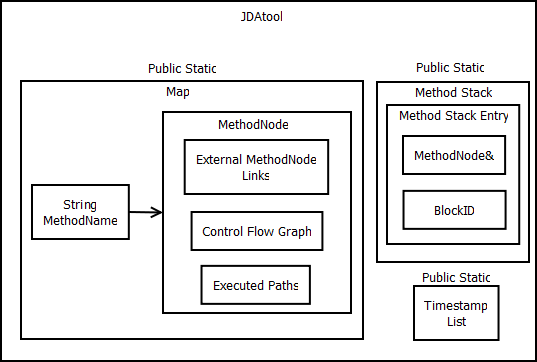
\includegraphics[width=0.48\textwidth]{JDAtool.png}
  \caption{JDA's Object Heirarchy}
  \label{fig:JDAtool}
\end{figure}

\subsection{MethodNode}
The core of all method information resides in the MethodNode class.
Every unique method tag (which includes overloaded methods) reserves its own persistent MethodNode.
The MethodNodes reside in the JDAtool in a Map.
The Map allows the String typed method tags to access their respective MethodNodes.

MethodNode contains three vital pieces of information: a Control Flow Graph (CFG), a Set of ExternalLinks, and a Set of BasicBlockPaths.
The CFG contains information regarding the control flow of bytecode basic blocks in the method.
This is analyzed when the class is first loaded.
The Set of ExternalLinks contains method invocation information within that MethodNode.
They essentially keep track of the MethodNode’s basic blocks in the CFG that call other MethodNodes.
This allows us track method invocations of any sort, including invokedynamic calls.

The final data structure is the Set of BasicBlockPaths.
A method’s instrumentation can track the basic blocks that any single invocation executes.
The blocks are concatenated together to form a BasicBlockPath.
However, the BasicBlockPath implementation is somewhat unfinished; while it can recognize identical paths, it does not include loop detection.
Large or unbounded loops within a method can become very burdensome in memory with this implemetation.
As such, the option for path tracking, trackPaths, may be disabled.

\subsection{MethodStack}
The method stack is simple a list of MethodStackEntrys (MSE), where each MSE contains a MethodNode reference and an integer block ID.  
Every time a new bytecode basic block is executed, the block ID is updated.  
Every time a new method is called, that method creates a new MSE with its own MethodNode reference and adds it to the stack.  
With the MethodStack and block ID updates in each MSE, methods can extrapolate what other methods called them.  
They can then update the caller’s MethodNode with a now known ExternalLink.  
In order to track ExternalLinks, the trackBlocks option must be enabled.

\subsection{TimestampList}
The TimestampList (TLS) is essentially a list of time blocks that do not include instrumentation at the beginning and end of methods.
The TSL has a start and stop function that is used to record method execution.
When the TSL is told to start, it will record the current time.
When the TSl is told to stop, it will push onto the list the difference from the start time and the current time.

Since methods have fairly significant instrumentation at the beginning and end of their code blocks, it is necessary to ensure that the timing statistics do not include these instrumentation sections.
At the beginning of every method, the TSL is given a stop command which pushes the current time difference onto the list.
The instrumentation at the beginning of the method can then be executed without impacting the overall time.
After the beginning instrumentation, the TSL is given the start command again.

The end of the method follows a very similar routine.
The stop command is first called at the end of the method so that the method's native code timing is added to the TSL.
At this point, there is a small memory optimization that can potentially save lots of memory being consumed by the TSL.
The methods store the current index of the TSL at the beginning of the method.
At the end of the method, they can add all of the times from that index to to the current index, remove those TSL entries, and add the final time to the list.
If the method does not call any other methods, then this optimization does nothing since there is only one new TSL entry since the beginning of that method.
However, methods that do call other methods will have lots of sparse timing entries that can be combined.
The pruning is done at the end of every method to reduce the memory complexity of the TSL.

The noise, granularity, and odd JIT optimizations make the accuracy of the TSL questionable for smaller methods, however large methods behave appropriately.
Additionally, The feature can be turned on by setting the trackTimes option.
Aside from timing small functions, the only other caveat to timing statistics is that they do not exclude the basic block instrumentation.
There is still instrumentation at the beginning of bytecode basic blocks if block tracking is turned on, however it is too fine grained to exclude from timing.

\section{JUNG Library}
All of the instrumentation gathers data into the JDAtool class, however the purpose of this tool is to graphically show the harvested information.
We investigated different Java CFG libraries and decide to use JUNG as the framework to build our GUI \cite{JUNG}.
JUNG, the Java Universal Network/Graph Framework, is a software library that provides a common and extendible language for the modeling, analysis, and visualization of data that can be represented as a graph or network.
The JUNG library provides powerful graph representation and easily customized graph APIs.
In our GUI, we used the mouse listener, vertex/edges render/transformer along with Java build-in javax.swing package to realize most of the functionalities. 

\section{GUI}
The GUI is launched at the end of the main function of the instrumented program, which ensures that the launch of the GUI will not interfere with the instrumention or add jitter to the runtime statistics.
The main purpose of the GUI is to enable better interpretation of the statistics that JDA generates.
In fact, almost all of the information that the JDA analyzes are related to Control Flow Graph vertices and edges.
A graphical interface with control flow graph is allows the user to interpret the gathered data in an organized fashion.
A lot of information can be shown in a macroscopic manner immediately after the rendering of the control flow graph. 
This includes the locations of active nodes, code coverage, edge weight, and related timing statistics.
On the other hand, more detailed information is accessable by text area output in the GUI invoked by mouse listeners, which facilitates the search for certain statistics the user cares about such as method invocations and pathing.

We designed every MethodNode to launch its own GUI so that the individual GUIs are only responsible for small chunks of data as well as allowing the user to swap between MethodNodes easily.
The main chanllenge in the GUI is to provide a stable layout for the control flow graph.
When it comes to graph layout, there are numerous layout algorithms to fulfill various constraints.
For instance, JUNG  KK layout, FR layout, and tree layout algorithms.
In our application, the graph we are looking at is the control flow graph with potentially complex structures.
Devising an algorithm that produce efficient and clean CFG layout becomes the main problem.
There are three main requirements for the layout: no overlapping in nodes or edges, space efficient, and the flow goes in top-down direction.

Algorithm \ref{alg1} is the algorithm we use to position the control flow graph.
this algorithm generates a non-overlapping layout in $O (V+E)$ time complexity.
It is based on a breadth-first search (BFS) algorithm \cite{kamada1989algorithm}.
When designing the layout algorithm, we make the decision to only expand the graph in width to the right, which lowers space consumption but is prone to more overlapping.
We solve this problem by expanding the ancestors when there exsists branches in successors.
The caveat is that the graph will easily expand to a large size in width given a branchy input if we always use the indentation as the summation of successors.
To avoid this, we can reset the indentation as we see a vertex that has only one child.
For example, vertex 4\ in the graph as shown in Figure \ref{eg1} has successor 6 which has 3 children.
As long as there is no other branch within two levels (vertex 6 is the only child of vertex 4) then we can reset the indentation of vertex 4\ in upper level.

Figure \ref{dm1} shows the comparison between our algorithm and other main stream solution to CFG layout.
All four CFGs have the same structure.
The only difference is our algorithm does not make the start block and return block a separate one, and we forced the block with the return statement to the bottom.
Comparison shows our algorithm saves more space in both width and height even with modest inputs.
Additionally, our algorithm doesn't compromise the clear interpretation of the control flow.

\begin{figure}[h]
\center
  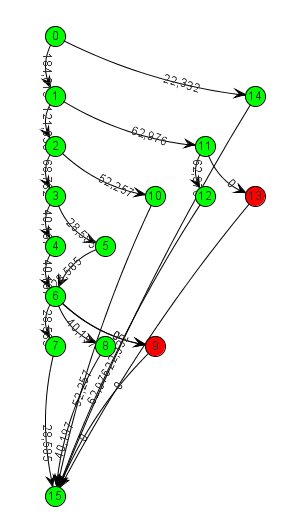
\includegraphics[width=0.5\textwidth]{layout_demo2.png}
  \caption{Indentation of our algorithm}
  \label{eg1}
\end{figure}

\begin{figure}[h]
\center
  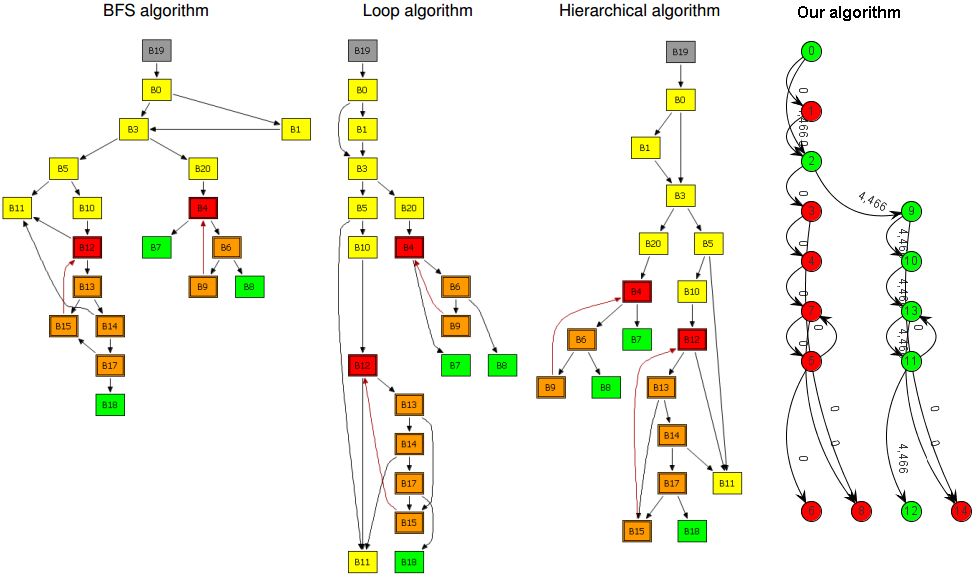
\includegraphics[width=0.5\textwidth]{layout_demo.png}
  \caption{Comparison of different layout algorithms}
  \label{dm1}
\end{figure}

\begin{algorithm}                      % enter the algorithm environment
\caption{CFG layout}          % give the algorithm a caption
\label{alg1}                           % and a label for \ref{} commands later in the document
\begin{algorithmic}[1]               % enter the algorithmic environment

    \REQUIRE $G=(V,A)$\\ $\exists !\ start \in V,\ s.t.\ Indegree(start)=0,$\\ $\exists\ E \in V,\   s.t. \ \forall \ end \in E, \ Outdegree(end)=0$
    \ENSURE $Postion(G),\ \forall\ v\in V, \ \not\exists \ v,\ v' \in V,\  v \not= v'$\\$\ s.t. \ Position(v)=Position(v')$\\
    \STATE $start \Leftarrow initpos(initx,inity)$
\STATE $Visited$  $\cup \Leftarrow start$
\STATE $N \Leftarrow SortedSuccessors(start)$
 \STATE $maxWidth,\ maxDepth\  \Leftarrow$\\$SuccessorLayout(N,\ initx,\ inity+\Delta y,\ Visited)$ 
    \FORALL{$end \in E$}
      \STATE $end \Leftarrow endpos(initx,inity+maxDepth+\Delta y)$
       \STATE $Next$	
        \STATE $initx \Leftarrow initx+\Delta x$
    \ENDFOR
\RETURN
\end{algorithmic}

\begin{algorithmic}
\STATE $ SuccessorLayout$
\end{algorithmic}


\begin{algorithmic}[1]
 \REQUIRE $N,\ width,\ depth,\ Visited$
    \ENSURE $maxWidth,\ maxDepth$\\
        \IF{$N = \{\}$}
           \RETURN $width,\ depth$
        \ELSE
            \STATE $newdepth \Leftarrow depth$
            \STATE $successorCount \Leftarrow 0$
\FORALL{$n \in N$}
	\IF{$n \not\in Visited$}
	\STATE $continue$
	\ENDIF
	\STATE $Visited$  $\cup \Leftarrow n$
	\STATE $n \Leftarrow initpos(width,depth)$
	\STATE $maxWidth,\ maxDepth\  \Leftarrow$\\$SuccessorLayout(N,\ width,\ depth+\Delta y,$\\$Visited)$
       \STATE $Next$	
	\STATE $newdepth \Leftarrow$\\$MAX(newdepth, maxDepth)$
	\STATE $width \Leftarrow$\\$width+\Delta x * (OutDegree(n)+maxWidth)$
	\STATE $successorCount \Leftarrow$\\$successorCount + OutDegree(n)-1$ 
\ENDFOR
	\IF{$size(N) = 1$}
	\STATE $maxWidth \Leftarrow 0$
	\ELSE
	\STATE $maxWidth \Leftarrow successorCount$
        \ENDIF
        \STATE $maxDepth \Leftarrow newDepth$
        \RETURN  $maxWidth,\ maxDepth$
\ENDIF
\end{algorithmic} 
\end{algorithm}

As shown in Figure \ref{gui}, our GUI pops out after the instrumentation program finishes.
It will show the CFG of each method in the class with different colors indicating node activeness and size indicating whether there is method call in that node.
Edges are filled with number of executions of all the path that pass through this edge.
The mouse listeners have two modes: transforming and picking.
In transforming mode, users can drag, rotate, zoom in/out the whole graph.
In picking mode, users can click on a certain node to see the statistics in the textarea and see the path that go through that nodes one by one.
On the control panel, the user can change the type and offset of the edges to render the graph, reset the graph, choose mouse modes as well as filter out infrequent nodes/path by input a threshold.
An examiner lens is also provided to see the details of the graph for more complex CFGs.

\begin{figure*}[t]
\center
  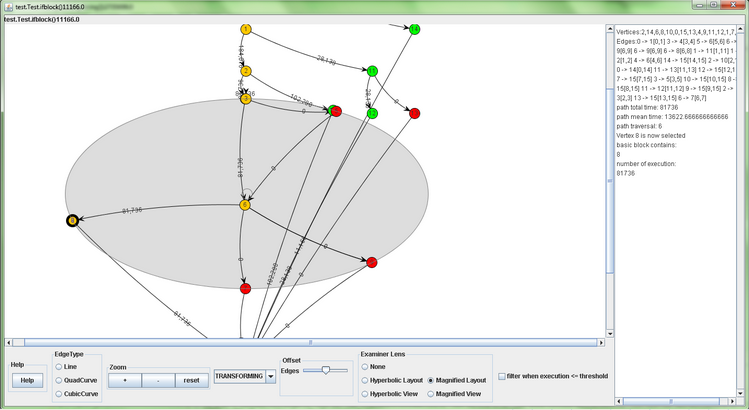
\includegraphics[width=\textwidth]{gui.png}
  \caption{GUI window}
  \label{gui}
\end{figure*}

\section{Future Work}
There is a good deal of improvement that can be made to the JDA’s path tracking features.
Namely, the implementation of loop detection in paths.  
Ideally, paths should be pruned at the exit of methods by compressing loops into special subpaths.  
Loops can be simply made up of single paths or contain numerous branch statements which makes the control flow analysis hard to sort.  
There are various ways to hash loops, and thus the hashing method should be configurable.  
The concept of the JDA was more focused around tracking virtual method invocations, however the baseline instrumentation is already in place for more complex analysis.

\section{Conclusion}
Other profiling tools tend to specialize in certain niche areas, and they actually perform better than JDA for these situations.
Similar to other profiling tools, JDA can learn different statistics about a program during runtime via instrumentation.
However, JDA is a tool that embraces a broad number of profiling concepts such as code coverage and performance timing in a single tool.
JDA also provides the lower level bytecode basic block pathing and coverage information that is not included in other source code coverage tools.
The pathing also extends beyond local method CFGs by tracking additional method calls like $invokevirtual$ through a method stack.
Additionally, The various types of instrumentation can be toggled with different inputs into the javaagent.
At the end of the instrumented program, an informative GUI is launched to graphically and interactively show all of the information.
JDA can be a great help to software developers to quickly determine if tests cover the bytecode sections that they want while providing additional information to aid their development.

\bibliographystyle{./IEEE/IEEEtran}
\bibliography{report.bib}
\end{document}
